\documentclass{article}
\usepackage{pgfplots}
\usepackage{enumitem}
\usepackage{fancyhdr}
\usepackage{extramarks}
\usepackage[english]{babel}
\usepackage{amsthm}
\usepackage{amsfonts}
\usepackage[T1]{fontenc}
\usepackage[plain]{algorithm}
\usepackage{algpseudocode}
\usepackage{xcolor,listings}
\usepackage{textcomp}
\usepackage{tabularx}
\usepackage{geometry}
\usepackage{booktabs}
\usepackage{hyperref}
\usepackage{tikz}
\usepackage{venndiagram}
\usepackage{amsmath, amssymb}
\usepackage{graphicx}
\usepackage{marvosym}
\usepackage{listings,lstautogobble}

\lstnewenvironment{javacode}[1][]
{
    \lstset{
        language=Java,
        basicstyle=\small\ttfamily,
        keywordstyle=\color{blue},
        commentstyle=\color{green!40!black},
        stringstyle=\color{red},
        numbers=left,
        numberstyle=\tiny\color{purple},
        stepnumber=1,
        numbersep=10pt, % Adjusted to move line numbers outside the box
        frame=single,
        linewidth=\linewidth,
        breaklines=true,
        breakatwhitespace=false,
        tabsize=4,
        autogobble=true,
        xleftmargin=0pt, % Adjusted to start from the left margin within the box
        #1 % Options passed to lstset
    }
}
{}

\geometry{a4paper, margin=1in}
\usetikzlibrary{er}
\lstset{upquote=true}
\pgfplotsset{compat=1.18}
\usetikzlibrary{positioning,shapes}
\usetikzlibrary{positioning, arrows.meta}
\usetikzlibrary{automata,positioning}


%
% Basic Document Settings
%

\topmargin=-0.45in
\evensidemargin=0in
\oddsidemargin=0in
\textwidth=6.5in
\textheight=9.0in
\headsep=0.25in

\linespread{1.1}

\pagestyle{fancy}
\lhead{\hmwkAuthorName}
\chead{\hmwkClass}
\rhead{\firstxmark}
\lfoot{\lastxmark}
\cfoot{\thepage}

\renewcommand\headrulewidth{0.4pt}
\renewcommand\footrulewidth{0.4pt}

\setlength\parindent{0pt}

%
% Create Review Sections
%

\newcommand{\enterReviewHeader}[1]{
    \nobreak\extramarks{}{Review \arabic{#1} continued on next page\ldots}\nobreak{}
    \nobreak\extramarks{Review \arabic{#1} (continued)}{Review \arabic{#1} continued on next page\ldots}\nobreak{}
}

\newcommand{\exitReviewHeader}[1]{
    \nobreak\extramarks{Review \arabic{#1} (continued)}{Review \arabic{#1} continued on next page\ldots}\nobreak{}
    \stepcounter{#1}
    \nobreak\extramarks{Review \arabic{#1}}{}\nobreak{}
}

\setcounter{secnumdepth}{0}
\newcounter{partCounter}
\newcounter{reviewProblemCounter}
\setcounter{reviewProblemCounter}{1}
\nobreak\extramarks{Review \arabic{reviewProblemCounter}}{}\nobreak{}

%
% Review Problem Environment
%
% This environment takes an optional argument. When given, it will adjust the
% review counter. This is useful for when the problems given for your
% assignment aren't sequential. See the last 3 problems of this template for an
% example.
%
\newenvironment{reviewProblem}[1][-1]{
    \ifnum#1>0
        \setcounter{reviewProblemCounter}{#1}
    \fi
    \section{Review \arabic{reviewProblemCounter}}
    \setcounter{partCounter}{1}
    \enterReviewHeader{reviewProblemCounter}
}{
    \exitReviewHeader{reviewProblemCounter}
}

%
% Homework Details
%   - Title
%   - Due date
%   - Class
%   - Section/Time
%   - Instructor
%   - Author
%
\newcommand{\rectangle}{\rule{0.5em}{0.5em}}
\newcommand{\hmwkTitle}{}
\newcommand{\hmwkDueDate}{19.06..2024}
\newcommand{\hmwkClass}{Wissenschaftliches Arbeiten}
\newcommand{\hmwkClassInstructor}{Prof. Dr.-Ing. Klaus Berberich /Prof. Dr. Peter Birkner}
\newcommand{\hmwkAuthorName}{\textbf{Yahya E. Selo}}

%
% Title Page
%

\title{
    \vspace{3in}
    \textmd{\textbf{\hmwkClass}}\\
    \normalsize\vspace{0.2in}\small{Due\ on\ \hmwkDueDate\ at 18:00}\\
    \vspace{0.2in}\large{\textit{\hmwkClassInstructor}}
    \vspace{3in}
}

\author{\hmwkAuthorName}

\renewcommand{\part}[1]{\textbf{\large Part \Alph{partCounter}}\stepcounter{partCounter}\\}

%
% Various Helper Commands
%

% Useful for algorithms
\newcommand{\alg}[1]{\textsc{\bfseries \footnotesize #1}}

% For derivatives
\newcommand{\deriv}[1]{\frac{\mathrm{d}}{\mathrm{d}x} (#1)}

% For partial derivatives
\newcommand{\pderiv}[2]{\frac{\partial}{\partial #1} (#2)}

% Integral dx
\newcommand{\dx}{\mathrm{d}x}

% Alias for the Solution section header
\newcommand{\solution}{\textbf{\large Solution}}

% Probability commands: Expectation, Variance, Covariance, Bias
\newcommand{\E}{\mathrm{E}}
\newcommand{\Var}{\mathrm{Var}}
\newcommand{\Cov}{\mathrm{Cov}}
\newcommand{\Bias}{\mathrm{Bias}}

\begin{document}


\maketitle


\pagebreak
\tableofcontents


\pagebreak
\begin{reviewProblem}
    \section{Einleitung}
    
    Der Blue Screen of Death (BSOD) ist ein bekanntes und gefürchtetes Problem in der Welt der Windows-Betriebssysteme. Er tritt auf, wenn das Betriebssystem auf einen schwerwiegenden Fehler stößt, von dem es sich nicht erholen kann. Dieser Fehler zwingt das System, sofort anzuhalten, und zeigt einen blauen Bildschirm mit einer Fehlermeldung an. BSODs sind besonders problematisch, da sie oft ohne Vorwarnung auftreten und dazu führen können, dass ungespeicherte Daten verloren gehen und Arbeitsprozesse abrupt unterbrochen werden.
    
    Das Auftreten eines BSOD kann auf eine Vielzahl von Problemen zurückzuführen sein, darunter Hardwarefehler, fehlerhafte Treiber, inkompatible Software oder sogar Malware-Infektionen. Die Fehlermeldung auf dem blauen Bildschirm enthält häufig einen Fehlercode, der auf die zugrunde liegende Ursache hinweisen kann, jedoch erfordert die genaue Diagnose und Behebung des Problems oft umfassende Kenntnisse und spezialisierte Werkzeuge.
    
    Dieser Bericht zielt darauf ab, das Problem des BSOD detailliert zu untersuchen, verschiedene Ursachen und deren Lösungen zu analysieren und einen Überblick über bestehende Diagnose- und Behebungsmethoden zu geben. Zudem werden innovative Ansätze und Technologien vorgestellt, die zur Vermeidung oder schnellen Behebung von BSODs beitragen können.
    
    \begin{figure}[!ht]
        \centering
        \begin{minipage}[b]{0.4\textwidth}
            \centering
            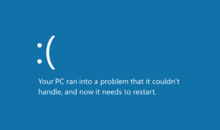
\includegraphics[width=\textwidth]{Pic/day 2/220px-Blue_Screen_of_Death.png}
            \caption{Blue Screen of Death}
            \label{fig:image}
        \end{minipage}
        \hfill
        \begin{minipage}[b]{0.4\textwidth}
            \centering
            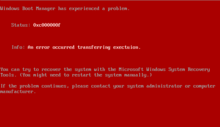
\includegraphics[width=\textwidth]{Pic/day 2/220px-Red_Screen_of_Death.png}
            \caption{Red Screen of Death}
            \label{fig:image_two}
        \end{minipage}
        \vfill
        \begin{minipage}[b]{0.4\textwidth}
            \centering
            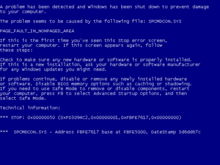
\includegraphics[width=\textwidth]{Pic/day 2/220px-Windows_XP_BSOD.png}
            \caption{Windows XP BSOD}
            \label{fig:image_three}
        \end{minipage}
        \hfill
        \begin{minipage}[b]{0.4\textwidth}
            \centering
            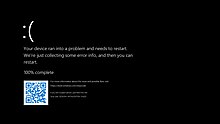
\includegraphics[width=\textwidth]{Pic/day 2/Windows11BSOD.jpg}
            \caption{Windows11 BSOD}
            \label{fig:image_four}
        \end{minipage}
        \caption{BSOD?}
        \label{fig:images_img}
    \end{figure}
    
    \pagebreak
    
    \section{Hintergrund}
    
    Der Blue Screen of Death (BSOD) erschien erstmals in der Beta-Version von Windows 1.0. Wenn Windows eine andere DOS-Version als erwartet fand, zeigte es die Fehlermeldung "Incorrect DOS version" und andere Textnachrichten an. In der finalen Version von Windows 1.01 trat nach der Entfernung dieser zusätzlichen Nachrichten ein Fehler auf, der zufällige Zeichen nach der "Incorrect DOS version"-Nachricht druckte.
    
    Windows 2.0 und 2.1 verhielten sich ähnlich wie Windows 1.0 und kehrten bei einem Absturz oder kritischen Fehler zu DOS zurück. Windows 3.0 zeigte wichtige Systemmeldungen im Textmodus an, während Windows 3.1 den Hintergrund dieser Meldungen von schwarz auf blau änderte und beim Drücken von Strg+Alt+Entf einen einfachen Task-Manager anzeigte. Bei schwerwiegenden Fehlern kehrten auch diese Versionen zu DOS zurück.
    
    Der erste echte BSOD erschien in Windows NT 3.1 (1993) und wurde seitdem in allen nachfolgenden Windows-Betriebssystemen integriert. Ursprünglich starteten die Fehlermeldungen mit "*** STOP:", weshalb sie als "Stop-Fehler" bekannt wurden.
    
    BSODs können durch schlecht programmierte Gerätetreiber oder fehlerhafte Hardware verursacht werden, z.B. defekten Speicher, Probleme mit der Stromversorgung, Überhitzung oder Hardware, die außerhalb ihrer Spezifikationsgrenzen betrieben wird. In den Windows 9x-Betriebssystemen konnten auch inkompatible DLLs oder Fehler im Betriebssystemkern zu BSODs führen. Aufgrund der Instabilität und des fehlenden Speicherschutzes in den Windows 9x-Betriebssystemen traten BSODs dort häufiger auf.
    Im Gegensatz zur landläufigen Meinung verwendet die Windows Embedded Compact (ehemals Windows CE) Linie der eingebetteten Betriebssysteme keinen Blue Screen of Death.
    \begin{figure}[!ht]
        \centering
        \begin{minipage}[b]{0.4\textwidth}
            \centering
            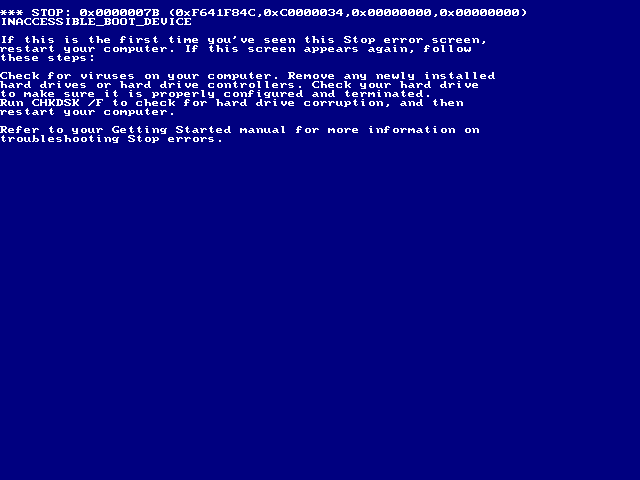
\includegraphics[width=\textwidth]{Pic/029-bsod_Windows_2000.png}
            \caption{Caption for image 1}
            \label{fig:image1}
        \end{minipage}
        \hfill
        \begin{minipage}[b]{0.4\textwidth}
            \centering
            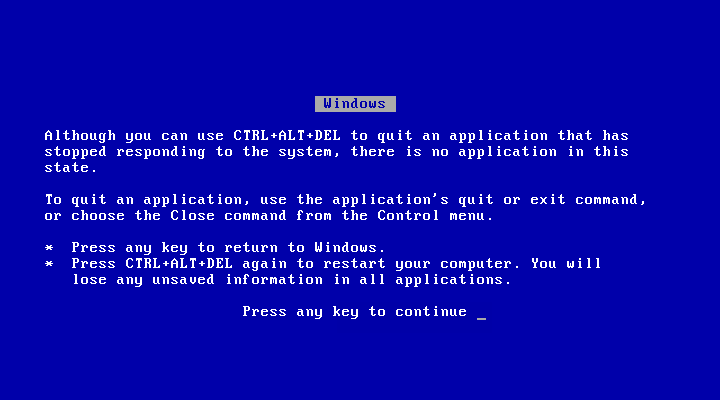
\includegraphics[width=\textwidth]{Pic/Windows_3.1_BSoD_(fixed).png}
            \caption{Caption for image 2}
            \label{fig:image2}
        \end{minipage}
        \vfill
        \begin{minipage}[b]{0.4\textwidth}
            \centering
            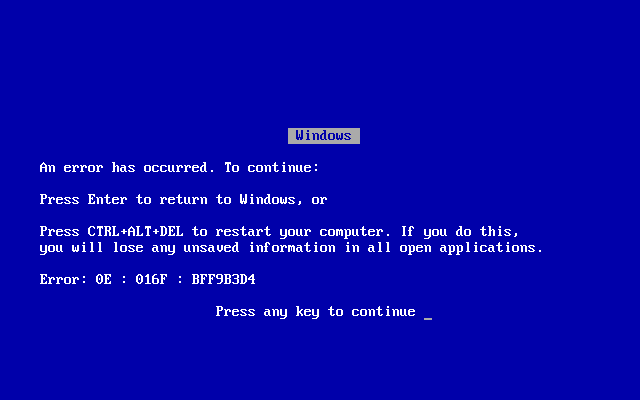
\includegraphics[width=\textwidth]{Pic/Windows_9X_BSOD.png}
            \caption{Caption for image 3}
            \label{fig:image3}
        \end{minipage}
        \hfill
        \begin{minipage}[b]{0.4\textwidth}
            \centering
            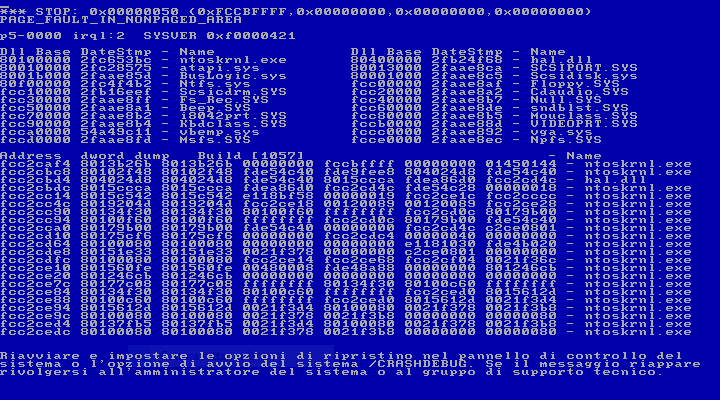
\includegraphics[width=\textwidth]{Pic/Windows_NT_3.51_BSOD_ita.png}
            \caption{Caption for image 4}
            \label{fig:image4}
        \end{minipage}
        \caption{BSOD-Staat im Laufe der Geschichte}
        \label{fig:images}
    \end{figure}
    
    \pagebreak
    \section{Methode}
    
    In diesem Abschnitt wird der spezifische Ansatz zur Analyse des Blue Screen of Death (BSOD) beschrieben. Dabei wird auf die verschiedenen Arten von BSODs und deren häufigsten Ursachen eingegangen, wobei zwischen Hardware- und Softwareproblemen unterschieden wird.
    
    \subsection{Arten von BSODs}
    
    Der BSOD kann in verschiedenen Formen auftreten, je nach zugrunde liegendem Problem. Die häufigsten Arten von BSODs sind:
    
    \begin{itemize}
        \item \textbf{Stop-Fehler:} Diese Fehler treten auf, wenn das Betriebssystem einen schwerwiegenden Fehler entdeckt, von dem es sich nicht erholen kann. Typische Stop-Fehler-Codes sind z.B. \texttt{0x0000007B} (INACCESSIBLE\_BOOT\_DEVICE) oder \texttt{0x0000001E} (KMODE\_EXCEPTION\_NOT\_HANDLED).
        \item \textbf{Treiberfehler:} Diese Fehler werden durch inkompatible oder fehlerhafte Gerätetreiber verursacht. Beispiele sind \texttt{0x000000D1} (DRIVER\_IRQL\_NOT\_LESS\_OR\_EQUAL) und \texttt{0x000000EA}
              \\(THREAD\_STUCK\_IN\_DEVICE\_DRIVER).
        \item \textbf{Hardwarefehler:} Diese Fehler resultieren aus Problemen mit der Hardware, wie z.B. defektem RAM, fehlerhaften Festplatten oder überhitzten Komponenten. Beispiele sind \texttt{0x0000009C} (MACHINE\_CHECK\_EXCEPTION) und \texttt{0x00000050} (PAGE\_FAULT\_IN\_NONPAGED\_AREA).
        \item \textbf{Windows 11: Black Screen of Death?} In Windows 11 ist der BSOD größtenteils schwarz, außer dem blauen QR-Code, aber die Meldung ist im Wesentlichen dieselbe wie in früheren Versionen.
    \end{itemize}
    
    \subsection{Ursachenanalyse}
    
    Die Ursachenanalyse eines BSODs erfordert ein systematisches Vorgehen, um die genaue Quelle des Problems zu identifizieren. Der Prozess umfasst folgende Schritte:
    
    \begin{enumerate}
        \item \textbf{Fehlermeldung und Codes analysieren:} Die auf dem BSOD angezeigten Fehlercodes und Meldungen geben erste Hinweise auf die Ursache des Problems. Diese Informationen sollten notiert und in einschlägigen Datenbanken oder Dokumentationen nachgeschlagen werden.
        \item \textbf{Ereignisprotokolle überprüfen:} Das Windows-Ereignisprotokoll enthält detaillierte Informationen über Systemereignisse und Fehler. Durchsuchen Sie das Protokoll nach kritischen Ereignissen, die zeitlich mit dem Auftreten des BSODs übereinstimmen.
        \item \textbf{Treiber und Hardware testen:} Führen Sie Tests durch, um mögliche Hardwarefehler zu identifizieren, z.B. durch Überprüfen des RAMs mit \texttt{memtest86+} oder der Festplatten mit dem \texttt{chkdsk}-Befehl. Aktualisieren Sie Gerätetreiber oder installieren Sie sie neu, um Treiberprobleme auszuschließen.
        \item \textbf{Diagnosetools verwenden:} Nutzen Sie spezialisierte Diagnosetools wie den Windows Debugger (\texttt{WinDbg}) und das BlueScreenView-Tool, um detaillierte Informationen aus den Speicherabbilddateien (\texttt{.dmp}-Dateien) zu extrahieren und die Ursache des BSODs zu bestimmen.
    \end{enumerate}
    \pagebreak
    \subsection{Häufigste Ursachen für BSOD}
    
    Die häufigsten Ursachen für einen Blue Screen of Death auf Ihrem Windows-PC sind:
    
    \begin{itemize}
        \item \textbf{Treiber:} Computer-Treiber sind Dateien, die in der Regel von einem Hardwarehersteller entwickelt werden und die Hardware im Betriebssystem funktionsfähig machen. Laut Microsoft sind 70 % der Stop-Fehler auf Drittanbieter-Treiber zurückzuführen.
        \item \textbf{Software:} Inkompatible Software wie Apps oder Programme können Konflikte verursachen, die zu einem BSOD führen.
        \item \textbf{Hardware:} Fehlerhafter Speicher (RAM), Festplatten (HDD), Solid-State-Laufwerke (SSD), Mainboards, Prozessoren oder Netzteile (PSU) können alle für Blue Screen-Abstürze verantwortlich sein.
        \item \textbf{Überhitzung:} Ihr Computer kann den BSOD anzeigen, wenn er aufgrund von Staub, defekten Lüftern oder überlasteter Hardware überhitzt.
        \item \textbf{Malware:} Malware, wie ein PC-Virus, der Ihre wichtigen Dateien und Ordner beschädigt, kann der Grund für einen Blue Screen of Death sein.
    \end{itemize}
    
    \subsection{Verwaltung des BSOD in Windows}
    
    Wir können verhindern, dass Windows nach einem Blue Screen-Fehler automatisch neu startet, indem wir folgende Schritte ausführen: 
    \begin{itemize}
        \item Geben wir in der Windows -Suchleiste „Systemeigenschaften“ ein und drücken wir Enter.
        \item Suchen wir im Tab „Erweitert“ nach „Starten und Wiederherstellen“.
        \item Klicken auf Einstellungen und deaktivieren Sie die Option „Automatisch neu starten“ unter Systemfehler, um zu verhindern, dass Ihr PC nach dem BSOD automatisch neu startet.
        \item Hier können Sie auch festlegen, wie Windows ein Systemfehlerereignis im Systemprotokoll speichert.
    \end{itemize}
    
    
    \pagebreak
    
    \section{Evaluation}
    
    In diesem Abschnitt werden der vorgeschlagene Ansatz zur Analyse und Behebung des Blue Screen of Death (BSOD) mit anderen bestehenden Ansätzen verglichen und die Vor- und Nachteile der verschiedenen Methoden zur Diagnose und Lösung von BSOD-Problemen diskutiert.
    
    \subsection{Vergleich des Lösungsansatzes mit anderen bestehenden Ansätzen}
    
    Der vorgeschlagene Ansatz zur Diagnose und Behebung von BSOD-Problemen umfasst die systematische Analyse von Fehlercodes, die Überprüfung von Ereignisprotokollen, das Testen von Treibern und Hardware sowie die Nutzung spezialisierter Diagnosetools. Dieser Ansatz wird nun mit anderen bestehenden Methoden verglichen:
    
    \begin{itemize}
        \item \textbf{Manuelle Fehlersuche:} Traditionell wird die manuelle Fehlersuche verwendet, bei der Administratoren oder Techniker die auf dem BSOD angezeigten Fehlercodes und Meldungen untersuchen und in Dokumentationen nachschlagen. Diese Methode kann zeitaufwändig und fehleranfällig sein, erfordert jedoch keine speziellen Tools.
        \item \textbf{Automatisierte Diagnosetools:} Es gibt verschiedene automatisierte Tools wie BlueScreenView, WhoCrashed und Windows Debugger (WinDbg), die detaillierte Informationen aus Speicherabbilddateien extrahieren und mögliche Ursachen identifizieren können. Diese Tools können die Diagnose beschleunigen und genaue Informationen liefern, sind jedoch oft komplex in der Handhabung.
        \item \textbf{Proaktive Wartung:} Einige Ansätze setzen auf proaktive Wartung, bei der regelmäßig Treiber und Software aktualisiert, Hardwarekomponenten überprüft und Systemressourcen überwacht werden, um BSODs zu verhindern. Dies erfordert kontinuierliche Aufmerksamkeit und Ressourcen, kann jedoch dazu beitragen, Ausfälle zu minimieren.
    \end{itemize}
    
    \subsection{Diskussion der Vor- und Nachteile der verschiedenen Methoden}
    
    Jede der genannten Methoden zur Diagnose und Behebung von BSOD-Problemen hat ihre eigenen Vor- und Nachteile:
    
    \begin{itemize}
        \item \textbf{Manuelle Fehlersuche:}
              \begin{itemize}
                  \item \textbf{Vorteile:} Keine speziellen Tools erforderlich, flexibel anwendbar.
                  \item \textbf{Nachteile:} Zeitaufwändig, fehleranfällig, erfordert Expertenwissen.
              \end{itemize}
        \item \textbf{Automatisierte Diagnosetools:}
              \begin{itemize}
                  \item \textbf{Vorteile:} Schnelle und genaue Diagnose, detaillierte Informationen, erleichtert die Fehlersuche.
                  \item \textbf{Nachteile:} Komplex in der Handhabung, erfordert Schulung und Verständnis der Tools.
              \end{itemize}
        \item \textbf{Proaktive Wartung:}
              \begin{itemize}
                  \item \textbf{Vorteile:} Kann BSODs vorbeugen, verbessert die Systemstabilität, reduziert Ausfallzeiten.
                  \item \textbf{Nachteile:} Erfordert kontinuierliche Aufmerksamkeit und Ressourcen, nicht immer effektiv bei unvorhersehbaren Fehlern.
              \end{itemize}
    \end{itemize}
    
    \subsection{Wie behebt man einen Blue Screen of Death?}
    
    Ein gelegentlicher BSOD, den Sie nie wieder sehen, könnte harmlos sein. Regelmäßige Blue Screens können jedoch problematisch und frustrierend sein, da sie auf tiefere Probleme hinweisen und dazu führen können, dass Sie bei jedem Neustart Daten verlieren. Nach einem BSOD sind zwei Dinge zu beachten:
    
    \begin{itemize}
        \item Softwareprobleme aufgrund von schlechtem Code, Inkompatibilität oder Malware.
        \item Hardwareprobleme aufgrund von Inkompatibilität oder Schäden durch Stöße, Alterung oder Spannungsfluktuationen.
    \end{itemize}
    
    \textbf{Treiber:} Geben Sie „Nach Updates suchen“ in die Windows-Suchleiste ein, um Windows Update zu finden. Verwenden Sie diese Funktion, um Ihre Treiber und Software zu aktualisieren und die Stabilität zu verbessern. Neue Treiber können jedoch selten auch Systemfehler verursachen. Sie könnten versuchen, die Änderungen zurückzusetzen, wenn ein neuer Treiber BSOD-Probleme ausgelöst hat.
    
    \textbf{Schlechte Software:} Software, die nicht gut mit anderen Programmen harmoniert, kann Blue Screen Abstürze verursachen. Jede kürzlich heruntergeladene oder installierte Software könnte der Schuldige sein. Geben Sie „Programme hinzufügen oder entfernen“ in die Windows-Suchleiste ein, um die Einstellung „Apps und Features“ zu finden. Deinstallieren Sie hier die verdächtigen Programme. Sie können auch den abgesicherten Modus von Windows verwenden, wenn Sie aufgrund von Blue Screen Fehlern keine Software normal entfernen können.
    
    Alternativ können Sie die Systemwiederherstellungsfunktion verwenden, wenn Ihr Computer über Wiederherstellungspunkte verfügt. Geben Sie „Wiederherstellung“ in die Windows-Suchleiste ein und starten Sie die „Erweiterte Wiederherstellungstools“ aus der Systemsteuerung. Klicken Sie auf „Systemwiederherstellung öffnen“, um Ihr System auf einen potenziell stabileren Zustand zurückzusetzen.
    
    \textbf{Malware:} Viele verschiedene Arten von Malware, wie Computerviren, Computerwürmer, einige Trojaner und Ransomware, können einen BSOD verursachen, indem sie Ihre wichtigen Dateien beschädigen. Verwenden Sie einen kostenlosen Virus- und Malware-Scanner, um alle Arten von Malware zu finden und zu entfernen, um Ihr System zu reinigen.
    
    \textbf{Peripheriegeräte und neue Hardware:} Entfernen Sie alle Peripheriegeräte, die den BSOD verursachen könnten. Beginnen Sie damit, Drucker, Scanner, USB-Geräte und externe Speicher von Ihrem PC zu trennen. Entfernen Sie anschließend alle neuen Hardwarekomponenten. Wenn Sie beispielsweise einen neuen RAM-Riegel gekauft haben, verwenden Sie den alten. Wenn Sie eine neue Grafikkarte gekauft haben, wechseln Sie zurück zur vorherigen oder verwenden Sie die integrierten Grafikoptionen.
    
    Wenn nach dem Entfernen der nicht wesentlichen Hardware keine Blue Screen Fehler mehr auftreten, fügen Sie die Hardware nacheinander wieder hinzu, um das Problem zu isolieren. Panik ist nicht notwendig, wenn eine neue Hardware BSODs verursacht, da sie möglicherweise nicht fehlerhaft ist. Beispielsweise ist Ihr neuer RAM-Riegel möglicherweise nicht mit Ihrem Mainboard oder Ihrem anderen RAM-Riegel kompatibel. Ebenso kann eine perfekte Grafikkarte aufgrund von Konflikten, Treiberproblemen oder unzureichender Stromversorgung Abstürze verursachen.
    
    \textbf{Hardwaretests:} Sie können Ihren Speicher mit Windows- oder Drittanbieter-Tools auf Fehler überprüfen.
    \\ HCI Designs MemTest ist ein beliebtes Tool für RAM-Tests.
    \\ Suchen Sie alternativ nach „Windows-Speicherdiagnose“ in der Windows 10 Suchleiste.
    
    Verwenden Sie die Software Ihres Speicherlaufwerkherstellers, um Ihre Festplatte (HDD) oder Solid-State-Laufwerk (SSD) auf Fehler zu überprüfen. Hier sind einige schnelle Links für Samsung, Western Digital und Seagate.
    
    \pagebreak
    Achten Sie auf Artefakte oder langsame Computerreaktionen beim Spielen von Videospielen, um zu sehen, ob Ihre GPU fehlerhaft ist. Sie können auch Videospiel-Benchmarking-Tools verwenden, um Ihre Grafikkarte auf Defekte zu überprüfen.
    
    Ein fehlerhaftes Netzteil kann dazu führen, dass Ihr Computer überhitzt, spontan neu startet, langsamer wird, abstürzt oder den BSOD anzeigt. Die einfachste Möglichkeit, ein Netzteil zu testen, besteht darin, ein neues auszuprobieren.
    
    Überhitzung kann Blue Screen Fehler verursachen. Sie können ein Dienstprogramm wie Open Hardware Monitor verwenden, um die Temperaturen Ihrer CPU und GPU zu überprüfen. Ein Druckluftspray kann die Lüftungsschlitze und Lüfter in einem überhitzten Computer reinigen. Ihr System sollte auch gut belüftet sein, um kühl zu bleiben.
    
    \pagebreak
    \section{Fehlermeldungen in anderen Farben}
    
    \subsection{Windows 11 Black Screen of Death}
    In früheren Versionen von Windows 11 wurde der Bluescreen durch einen Blackscreen (schwarzen Bildschirm) ersetzt. Einige Monate nach der Veröffentlichung wurde die Farbe jedoch durch ein Update wieder durch dunkelblau ersetzt. Ein ähnliches Verfahren zeichnete sich ebenso in einigen Beta-Versionen von Windows 8 ab.
    
    \subsection{MS-DOS 6 Black Screen of Death}
    MS-DOS 6 ist das älteste Microsoft Betriebssystem, das den Blue Screen hat, jedoch wird er in der eingestellten Farbe des BIOS-Bildschirmtreibers (in der Regel Hellgrau auf Schwarz) angezeigt. Er wird von dem Treiber EMM386.EXE angezeigt, wenn im Protected Mode ein unbehandelter Prozessor-Interrupt (z. B. Segfault, Division by Zero) auftritt. Bei MS-DOS 5 wird in der gleichen Situation ein kritischer Fehler angezeigt, und dem Benutzer wird die Option gelassen, den Protected Mode zu beenden und zum DOS Befehlszeileninterpreter zurückzukehren, während MS-DOS 6 den „echten“ Bluescreen anzeigt, bei dem nur noch der Neustart möglich ist.
    \subsection{Windows 3.1 Black Screen of Death}
    In Windows 3.x erscheint der Black Screen of Death, wenn eine MS-DOS-Anwendung nicht richtig ausgeführt werden konnte. Sehr oft tritt dies auf, wenn man bestimmte Funktionen ausführt, während der Netzwerktreiber im Speicher aktiv ist. So beispielsweise während des Ladens des Novell-Netware-Clients NETX für MS-DOS: Das System versucht beim Auftreten des Fehlers in den Textmodus zu wechseln, zeigt aber nichts an, sodass der Anwender vor einem leeren schwarzen Bildschirm sitzt, auf dem in der linken oberen Ecke ein Cursor blinkt. Der Anwender kann zu diesem Zeitpunkt keine Eingaben mehr machen und ist gezwungen, einen Kaltstart des Systems durchzuführen, um weiterzuarbeiten.
    Laut Wallace McClure von ASP.net wurde der Ausdruck Black Screen of Death das erste Mal im Sommer 1991 von Ed Brown, einem IT-Techniker der Coca-Cola Company in Atlanta verwendet, der berichtete, dass die Angestellten des Unternehmens beim Versuch, WordPerfect zu starten, ab und zu einen Black Screen of Death erhielten.
    \subsection{Xbox 360 Black Screen of Death}
    Auf der Xbox 360 wird bei einem Generalfehler ein Schwarzer Bildschirm angezeigt und die Konsole kann nicht mehr verwendet werden. Auf dem Black Screen steht, man sollte den Xbox Support kontaktieren. Außerdem wird ein Fehlercode (z. B. E71, E64…) angezeigt. Der Kreis, auf dem normalerweise die Anzahl der angeschlossenen Controller angezeigt wird, leuchtet ein Viertel rot, ähnlich wie bei dem Red Ring of Death.
    \subsection{OS/2 Black Screen of Death}
    
    In OS/2 ist ein Black Screen of Death entweder ein TRAP Screen oder ein full-screen hard-error VIO pop-up. Beide sorgen dafür, dass die Anzeige in den Textmodus geschaltet wird. Diese Anzeige hat zur Darstellung des Textes 25 Zeilen mit je 80 Spalten, in denen weiße Buchstaben auf einen schwarzen Hintergrund dargestellt werden, woher diese Anzeige auch ihren Namen hat.
    \begin{itemize}
        \item \subsubsection{TRAP Screen}
              Ein TRAP Screen wird angezeigt, wenn im Kernel ein Fehler auftritt, der zur Laufzeit nicht korrigiert werden kann. Normalerweise passiert dies nach dem Übertakten von Hardware, aber auch bei Softwarefehlern im Kernel oder bei Gerätetreibern.
              
              Der TRAP Screen enthält dabei sowohl eine Auflistung der Prozessor-Register und des Stacks als auch Informationen über die Version des Betriebssystems und den aufgetretenen Fehler im Prozessor.
              
              Die einzige Möglichkeit, die der Anwender in dieser Situation hat, ist entweder ein Neustart des Systems durch den Klammergriff (gleichzeitiges Drücken von Strg + Alt + Entf), oder durch zweimaliges Drücken von Strg + Alt + Num Lock das System anzuweisen, alle Informationen aus dem Speicher auf Diskette zu speichern.
              
        \item \subsubsection{Hard Error Screen}
              Ein Full-screen hard-error VIO pop-up wird angezeigt, wenn ein Prozess einen schweren Fehler verursacht, entweder bei einem Absturz eines Programmes oder einem schweren Fehler, bei dem es möglich ist, das System wiederherzustellen, z. B. ausgelöst durch den Versuch, eine Diskette einzulesen, obwohl sich keine im Diskettenlaufwerk befindet.
              
              Diese Anzeige wird erstellt vom Hard-Error-Daemon-Prozess, der schwere Fehler von anderen Prozessen behandelt. Technisch betrachtet ist diese Anzeige eine VIO-pop-up-Anzeige. Alle Prozesse (ausgenommen derjenige, der den schweren Fehler ausgelöst hat) werden weiter ausgeführt. Dieser Daemon benutzt einen VIO-Pop-up, wenn entweder das System im Textmodus gestartet wurde oder wenn der Fehler in einem Prozess auftritt, der im Vollbildmodus läuft.
              
              Dieser Pop-up enthält Informationen über den aufgetretenen Fehler und den auslösenden Prozess.
              
              Der Anwender wird daraufhin gefragt, wie weiter vorgegangen werden soll. Er kann zwischen folgenden Aktionen wählen:
              
    \end{itemize}
    
    \begin{itemize}
        \item Prozess beenden
        \item Anzeige von mehr Informationen (Auflistung des Prozessor-Registers und des Stacks)
        \item Wiederholung der zum Fehler führenden Aktion (wenn möglich – z. B. sind I/O-Fehler wiederholbar, CPU-Fehler nicht)
        \item Ignorieren des Fehlers (wenn möglich – zum Beispiel sind I/O-Fehler ignorierbar, CPU-Fehler nicht).
    \end{itemize}
    
    \subsection{Red Screen of Death}
    Der Red Screen of Death (RSoD) ist eine Variante, der in einigen Beta-Versionen des Betriebssystems Windows Vista vorhanden war.
    
    Als Red Screen of Death werden außerdem auch fatale Fehler in neueren Versionen von Lotus Notes bezeichnet. Dort erscheint eine Fehlermeldung, aber nicht wie bei Windows Vista im Vollbildmodus, sondern als rote Box mit schwarzem Rahmen.
    \subsection{Andere Verwendungen}
    \begin{itemize}
        \item Der rote Bildschirm wird auch von einigen Flugsimulatoren (wie z. B. den von FlightSafety International) benutzt. Sobald ein Pilot das Flugzeug abstürzen lässt, wird jeder Bildschirm im Cockpit rot.
        \item Bei der PlayStation 2 wird dies auch zu folgender Fehlermeldung unterstützend verwendet: „DVD/CD-ROM im PlayStation- oder PlayStation-2-Format einlegen“. Dieser Fehler wird durch eine nicht unterstützte oder nicht lesbare Disk ausgelöst.
        \item Bei der PlayStation Portable tritt in sehr seltenen Fällen ein RSoD auf, wenn die flash0 (die interne Flash-Disk) beschädigt wird.
        \item Auf der SEGA Genesis / Mega Drive quittieren fehlerhaft gepatchte ROMs ihren Dienst mit einem Red Screen, welcher keinerlei Text enthält. Die Konsole muss in diesem Fall zurückgesetzt werden.
    \end{itemize}
    
    
    
    \pagebreak
    \section{Fazit}
    
    In diesem Bericht wurde die Problematik des Blue Screen of Death (BSOD) analysiert und verschiedene Ansätze zur Diagnose und Behebung dieser Probleme untersucht. Die wichtigsten Ergebnisse lassen sich wie folgt zusammenfassen:
    
    \begin{itemize}
        \item Der BSOD ist ein häufiges Problem, das durch eine Vielzahl von Ursachen wie Treiberprobleme, Softwareinkompatibilität, Hardwarefehler, Überhitzung und Malware verursacht werden kann.
        \item Verschiedene Diagnosemethoden, einschließlich manueller Fehlersuche, automatisierter Diagnosetools und proaktiver Wartung, bieten unterschiedliche Vor- und Nachteile bei der Identifizierung und Lösung von BSOD-Problemen.
        \item Die Evaluation ergab, dass automatisierte Diagnosetools wie BlueScreenView und WinDbg eine schnelle und präzise Fehlerdiagnose ermöglichen, während proaktive Wartungsansätze zur Vorbeugung von BSODs beitragen können, jedoch kontinuierliche Überwachung erfordern.
        \item Es wurde auch diskutiert, wie Nutzer durch einfache Schritte wie Treiberaktualisierungen, Softwarebereinigung und Hardwaretests die Wahrscheinlichkeit von BSODs reduzieren können.
    \end{itemize}
    
    Als mögliche nächste Schritte zur Verbesserung der BSOD-Diagnose und -Behebung könnten weitere
    \\ Forschungen in folgenden Bereichen angestrebt werden:
    
    \begin{itemize}
        \item Entwicklung fortschrittlicher Diagnosetools, die auch für nicht-technische Benutzer zugänglich sind.
        \item Integration von Künstlicher Intelligenz und maschinellem Lernen zur automatisierten Analyse von BSOD-Fehlern.
        \item Stärkere Zusammenarbeit zwischen Hardwareherstellern, Softwareentwicklern und Sicherheitsexperten, um die Stabilität und Kompatibilität von Systemkomponenten zu verbessern.
        \item Förderung von Bildungsprogrammen und Bewusstseinskampagnen, um Anwender über beste Praktiken bei der Vermeidung und Behebung von BSOD-Problemen aufzuklären.
    \end{itemize}
    
    Insgesamt zeigt dieser Bericht, dass die effektive Diagnose und Behebung von BSOD-Problemen durch eine Kombination aus technischen Kenntnissen, proaktiver Wartung und fortschrittlichen Diagnosetools möglich ist. Zukünftige Verbesserungen in diesen Bereichen könnten dazu beitragen, die Zuverlässigkeit und Benutzererfahrung von Computersystemen signifikant zu steigern.
    
    \clearpage
    % Hier beginnt das Literaturverzeichnis
    
    \section{Literaturverzeichnis}
    Hier werden alle zitierten Quellen und Referenzen aufgeführt
    \begin{itemize}[label=\rectangle]
        \item \textbf{So beheben Sie den Bluescreen of Death (BSOD) unter Windows 10 und 11}
              \begin{itemize}
                  \item \href{https://www.avast.com/de-de/c-how-to-fix-blue-screen-of-death}{Avast Academy}
              \end{itemize}
        \item \textbf{Resolving Blue Screen errors in Windows}
              \begin{itemize}
                  \item \href{https://support.microsoft.com/en-us/windows/resolving-blue-screen-errors-in-windows-60b01860-58f2-be66-7516-5c45a66ae3c6}{Microsoft Support}\\
                        Dies ist die Hauptseite des Microsoft-Supports, die die Probleme der Benutzer mit dem Bluescreen des Todes (Blue Screen of Death) behandelt.
              \end{itemize}
        \item \textbf{Bluescreen (Windows)}
              \begin{itemize}
                  \item \href{https://de.wikipedia.org/wiki/Bluescreen_(Windows)}{Bluescreen (Windows) wiki}\\
                        Hier ist die Wiki-Website, die über die verschiedenen Arten von Bluescreens des Todes (Blue Screen of Death, BSOD) spricht.
              \end{itemize}
        \item \textbf{Täglich 5 verschiedene Bluescreen.}
              \begin{itemize}
                  \item \href{https://answers.microsoft.com/de-de/windows/forum/all/t%C3%A4glich-5-verschiedene-bluescreen/e6d8caaf-75b6-4e9c-ae38-747884d1879d}{Microsoft Support}\\
                        Dies ist jedoch eine forum eines Benutzers und sein spezifisches BSOD-Problem.
              \end{itemize}
        \item \textbf{Malwarebytes What is BSOD}
              \begin{itemize}
                  \item \href{https://www.malwarebytes.com/cybersecurity/computer/blue-screen-of-death}{Malwarebytes}\\
                        Malwarebytes ist eine Anti-Malware-Software des im kalifornischen Santa Clara ansässigen Unternehmens Malwarebytes Inc. Sie ist für die Betriebssysteme Windows, macOS und Android verfügbar und, mit mehr als 100 Millionen Downloads, eine der verbreitetsten Anti-Malware-Lösungen. Im Jahr 2011 wurde das Unternehmen mit mehr als 20 Millionen Downloads als sechsthäufigster Download bei CNET ausgezeichnet.
              \end{itemize}
        \item \href{https://chatgpt.com/}{ChatGPT}
              
    \end{itemize}
    
    % Hier beginnt der Anhang
    \clearpage
    
    \section{Quellen}
    \href{https://www.google.com/url?sa=i&url=https%3A%2F%2Fwww.howtogeek.com%2F163452%2Feverything-you-need-to-know-about-the-blue-screen-of-death%2F&psig=AOvVaw2rDuoxLo7pbbeupebK0yOO&ust=1718897380151000&source=images&cd=vfe&opi=89978449&ved=0CBEQjRxqFwoTCIDM6O_954YDFQAAAAAdAAAAABAE}{Picture 1}\\
    \href{https://upload.wikimedia.org/wikipedia/commons/3/3b/Windows_9X_BSOD.png}{Windows 9X BSOD.png}\\
    \href{https://upload.wikimedia.org/wikipedia/commons/c/c1/BSoD_in_Windows_1.0.png}{BSoD in Windows 1.0.png}\\
    \href{https://upload.wikimedia.org/wikipedia/commons/6/61/Windows_NT_3.51_BSOD_ita.png}{Windows NT 3.51 BSOD ita.png}\\
    \href{https://upload.wikimedia.org/wikipedia/commons/4/44/Windows11BSOD.jpg}{Windows11BSOD.jpg}\\
    \href{https://upload.wikimedia.org/wikipedia/commons/2/22/Longhorn_RSoD.png}{RSoD.png}
\end{reviewProblem}

\end{document}
